\documentclass[12pt, a4paper]{article}
\usepackage{caption}
\captionsetup[figure]{name=Resim}
\usepackage{graphicx}
\renewcommand{\refname}{5  Kaynakçalar}
\graphicspath{ {./images/} }
%opening
\usepackage{url}
\title{ Yapay Zeka Dersi Proje Tasarım Raporu}
\author{Celal ALTIN}
\date{\today}

\begin{document}
	\textbf{KÜTAHYA SAĞLIK BİLİMLERİ ÜNİVERSİTESİ}\centering\\
	\textbf{Bilgisayar Mühendisliği}\centering
	\begin{figure}[!h]
		\centering
		
\includegraphics{ksbu.png}
	\end{figure}
	\thispagestyle{empty}
	
	\maketitle\raggedright
	\maketitle\raggedright
	\maketitle
Bu çalışma raporu vizeye kadar olan yapay zeka dersi çalışmalarımın detaylarını içermektedir.

\begin{enumerate} 
	\item Giriş
	\item Literatür Araştırması
	\item Metodoloji
	\item Kullanılacak Veriler
	\item Beklenen Sonuçlar %Sonuç
	\item Kaynakça
\end{enumerate}\raggedright
\newpage
\section{Giriş}
2019 yılında başlayan COVID-19 salgını dünya çapında ciddi sağlık, ekonomik ve sosyal etkilere yol açmıştır.(Mart 2022 de yayınlanan bir habere göre \cite{haber1} dünyada ölüm sayısının 18 milyonu aştığı hesaplanıyor, bu sayı ülkemizde ise Sağlık bakanlığının verilerine göre 31.05.2022 tarihine kadar 98.965 kişinin hayatını kaybetti yönünde.)Bugün bile bu etkilerin sonuçları geçmiş değildir.\\
\begin{figure}[!htbp]
	{
		\caption{Dunya Covit Haritasi \cite{site1}}
		\centering
		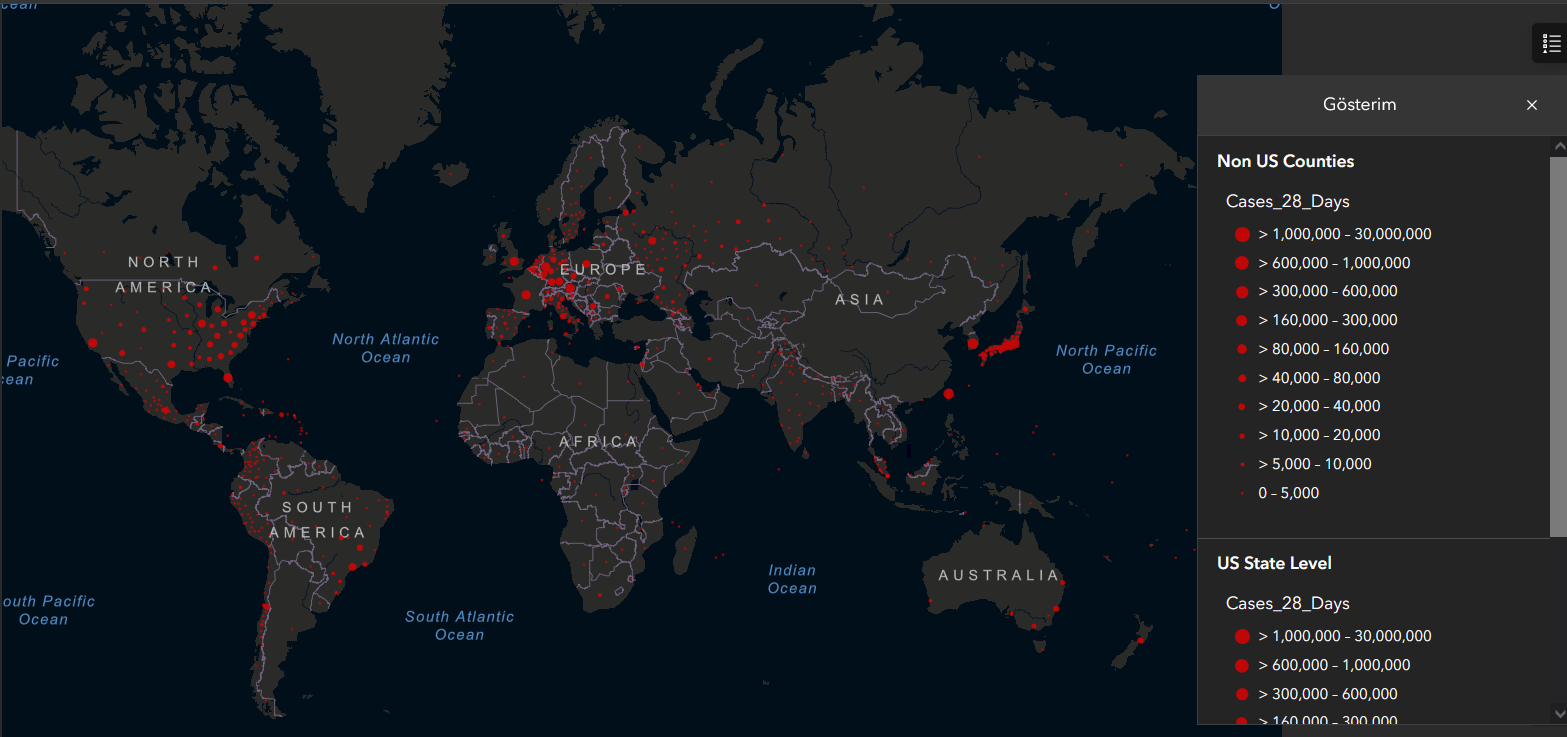
\includegraphics[angle=0, width=\textwidth]{hastalikdunya.png}
		\label{Dunya Covit Haritasi}
	}
	
	
\end{figure}
Dünya çapındaki bu problemi daha iyi anlayabilmek ve ileride olası hastalıklarda daha etkili mücadele edebilmek için bilgisayar(Makine öğrenmesi kulkanılarak yapılan bir araştırmaya göre sosyal medyanın da etkisiyle aşıya olan olumlu bakış artmıştır \cite{article} ) ve bilgisayar özelinde yapay zeka teknolojisinden faydalanmak en akılcı yöntemlerden birisidir.Bende bu projemde çeşitli kaynaklardan bulduğum Covit-19 verilerini kullanarak olası bir salgın hastalık dumunda gerçekleşebilecek seneryoyu gün yüzüne çıkartmayı amaçlıyorum.

\section{Literatür Araştırması}
Koronavirüs, 2019 yılının Aralık ayında ilk olarak Çin’in Wuhan kentinde ortaya çıkmış ve 11 Mart 2020’de Dünya Sağlık Örgütü tarafından pandemi olarak ilan edilmiştir. Vaka sayılarını kontrol altına almak için pek çok ülke karantina, sokağa çıkma yasağı ve sosyal alanların bir süreliğine kapatılması gibi çeşitli önlemler almıştır. Doğrulanmış vaka tahminlemesi pandemide olası planlamalar için büyük önem taşımaktadır. Gelecek verilerinin gerçeğe en yakın bir şekilde tahminlenmesi; pandemi döneminde lojistik, tedarik, hastane personel ve malzeme planlaması için kullanılabileceği gibi aşılama senaryolarında da girdi olarak kullanılabilir. Literatürde doğrulanmış vaka tahmininde makine öğrenmesi, bölmeli model, zaman serisi analizi gibi pek çok yöntem kullanarak tahminleme yapılan çalışmalar vardır. Bu çalışmada, Amerika Birleşik Devletleri’ndeki doğrulanmış vaka sayılarını kullanarak gelecek günlerdeki vaka tahminlerini çeşitli makine öğrenmesi modelleri yapılmıştır. Python ve R programlama dili kullanılarak yapılan tahminlemeler Prophet, Polinom Regresyon, ARIMA, Doğrusal Regresyon ve Random Forest modelleri ile yapılmıştır. Test verisiyle tahmin edilen verilerin performansları ortalama mutlak yüzde hatası (MAPE), ortalama karekök sapması (RMSE) ve ortalama mutlak hata (MAE) kullanılarak değerlendirilmiştir  \cite{article_855113}.\\ 
PCA(Veri boyutunu azaltma yöntemleri sınıflandırma yapmak için
harcanan zamanı ve bazı durumlarda sınıflandırma hatasını
azaltmaya yardımcı olur. Zaman kritik
uygulamalarda öznitelik elde etme evresinde harcanan zamanı
azaltmak için, öznitelik seçme yöntemleri, tüm giriş
değerlerinin ölçülmesini gerektiren boyut indirgeme
yöntemlerine tercih edilir\cite{genc2007new}) yöntemi kullanıldığında doğruluk değeri en yüksek RF algoritmasında,
duyarlılık ve kesinlik değeri en yüksek SMV algoritmasında saptanmıştır. Bu
yöntemin kullanılması sonucunda en düşük doğruluk NB algoritmasında,
duyarlılık ve kesinlik değerleri en düşük NB ve DT algoritmalarında elde
edilmiştir\cite{article_1031070}.
\begin{figure}[!htbp] 
	\caption{Dogruluk Tablosu}
	\centering
	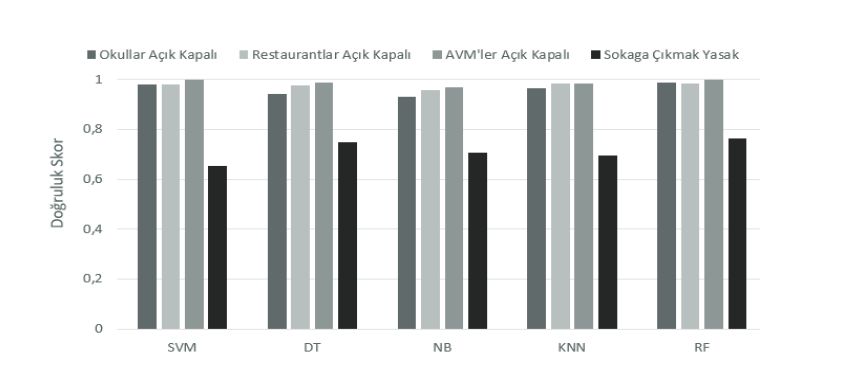
\includegraphics[angle=0, width=\textwidth]{dogruluk.png}
	\label{dogruluk}
\end{figure}
\newpage
\section{Metodoloji}
Projeni şematik planı aşağıdaki şekildedir.
\begin{figure}[!htbp]
	\caption{GANTT CHART}
	\centering
	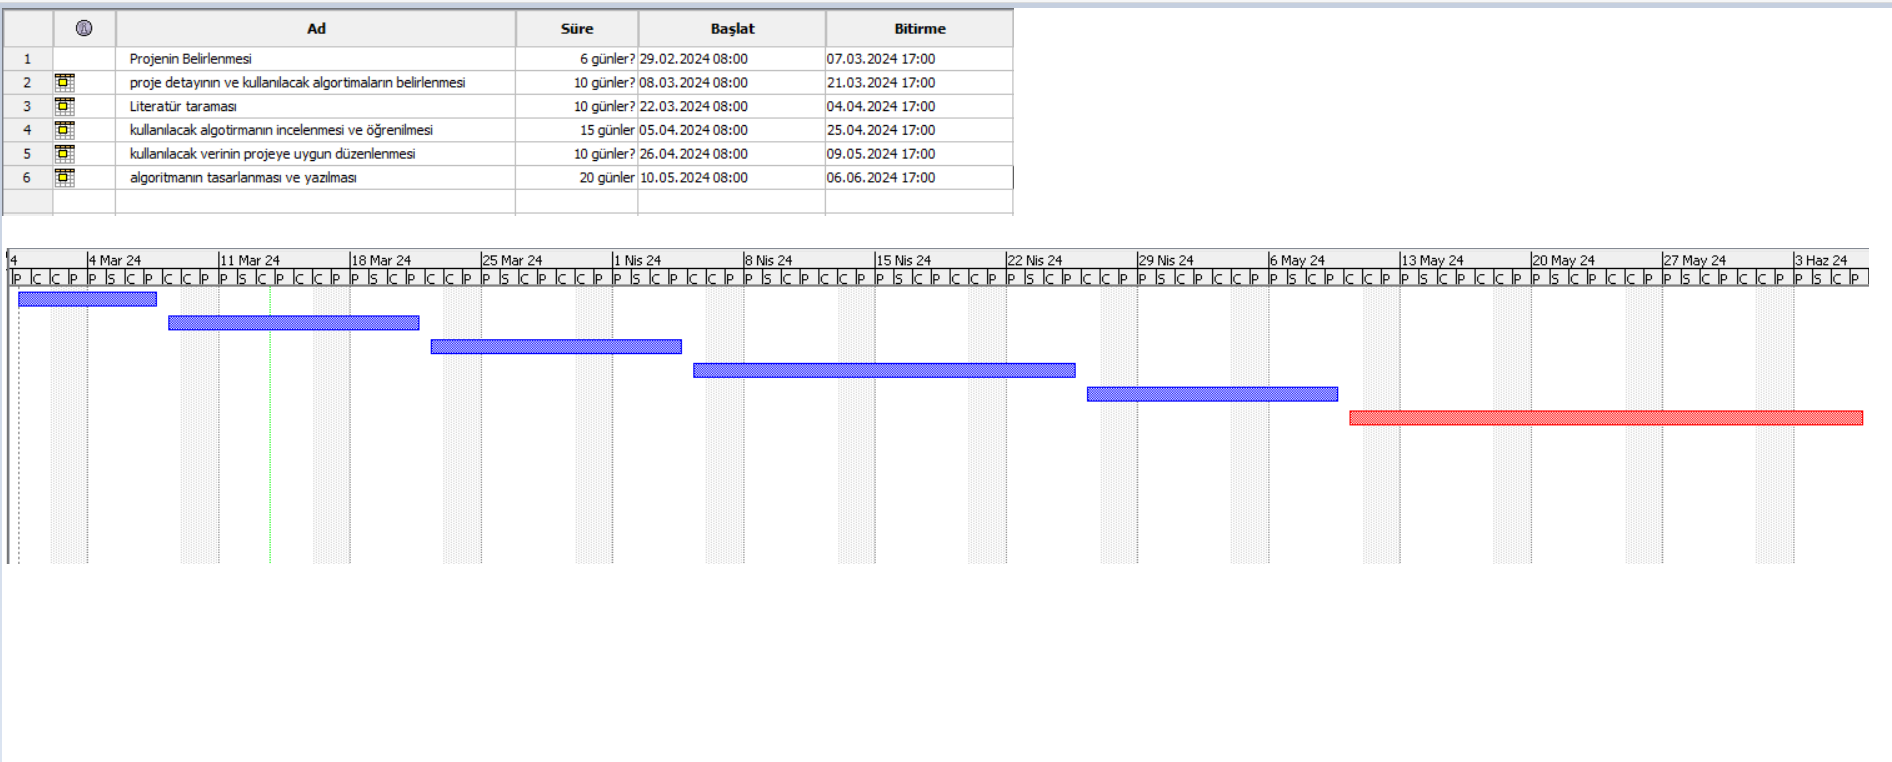
\includegraphics[ width=\textwidth]{gantt.png}
	\label{gantt}
\end{figure}

Projede kullanacağımız veriler gün veya haftalık olarak pozitif hasta sayısını, vefat edenlerin sayısını, kullandığımız verilerdeki insanların yaşadığı şehrin yada ülkenin nüfusunu, iyileşen sayısını,toplam test sayısı gibi parametreleri içermelidir.

Veri işleme
Normalizasyon işlemi- Araştırmalarda veri setlerinde verilerin
bütünlüğünün sağlanması, veri tekrarının önlenmesi ve veri bütünlüğünün
korunması ile performansının artırılması için normalizasyon yapılmaktadır.
Daha sonra Çapraz doğrulama (Çapraz doğrulama, makine öğrenimi
modellerinin başarı derecesini ortaya koymak için kullanılan yöntemdir.
Çapraz doğrulama algoritma performansı hakkında bilgi verirken, verilerin
daha verimli kullanılmasını sağlar.\cite{article_1031070})-yöntemi kullanılacaktır.
Daha sonra PCA yöntemi kullanılarak veri kümesini azalttıktan sonra RF(Random Forest) algoritmasına beslenecektir.

\section{Kullanılacak veri}

Projemde iki farklı veri kaynağından faydalandım.Bunlardan ilki T.C. Sağlık Bakanlığından alınmış verilerdir.\cite{siteSaglik}.Verilerimiz 11.03.2020-31.05.2022 tarihleri arasında alınmış 813 farklı kayda sahiptir.Bu veriler Toplam Vaka, Günlük Vaka, Toplam Hasta, Gunluk Hasta, Toplam Vefat, Gunluk Vefat, Toplam iyilesen, Gunluk iyilesen, Gunluk Test şeklinde etiketlenmiştir.  \newline İkinci olarak ise Our World in Data kaynağından faydalanılmıştır\cite{owidcoronavirus}.
\section{Beklenen Sonuçlar}
Olası bir salgın hastalık durumunda oluşabilecek sonuçları tahmin etmede fikir vermesi ve
projemin \% 90 nın üzerinde doğrulukla sonuçlanması.
\newpage
Çalışmamızda Random Forest algoritmasını kullanılacağından bahsedilmişti.Random Forest algoritması Denetimli Öğrenme algoritmaları sınıfına ait bir algoritmadır.İnternete Random Forest algoritması yazıldığında karşınıza Random Forest regresyon(Regression) ve Random Forest sınıflandırma (Classification) algoritmaları çıkacaktır.
\begin{figure}[!htbp] 
	\caption{ Machine Learning Algorithms }
	\centering
	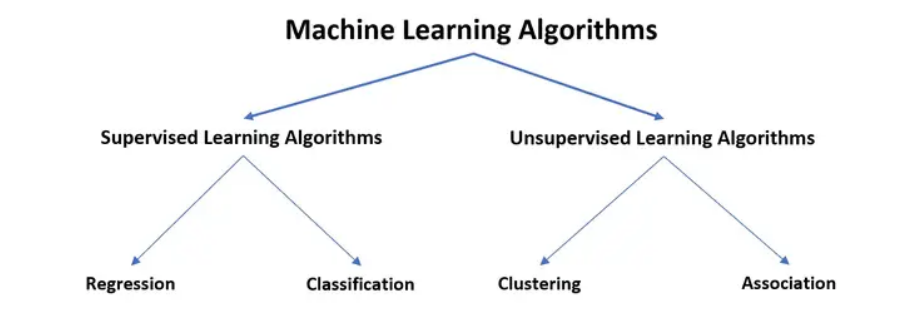
\includegraphics[angle=0, width=\textwidth]{resim3.png}
	
\end{figure} 
\newline Regresyon ve sınıflandırma farkından bahsetmeden önce denetimli öğrenme ve denetimsiz öğrenme algoritmaları arasındaki farktan bahsetmek daha sağlıklı olacaktır.\\
\textbf{Denetimli Öğrenme Algoritması:} Denetimli Öğrenme algoritmasındaki en önemli nokta etiketli bir veri kümesi (labeled dataset) kullanılmasıdır. Yani hangi verinin hangi bilgiye karşılık geldiği bilindiğinden bilinen bir girdi seti ile bunlara denk gelen çıktıları alıp algoritmanın daha önce hiç görmediği (eğitimde kullanılmayan) yeni verilere en uygun çıktıları üretmek için kullanılan bir makine öğrenmesi modelidir.\cite{site2}
\newpage
\begin{figure}[!htbp] 
	\caption{ Denetimli Öğrenme  }
	\centering
	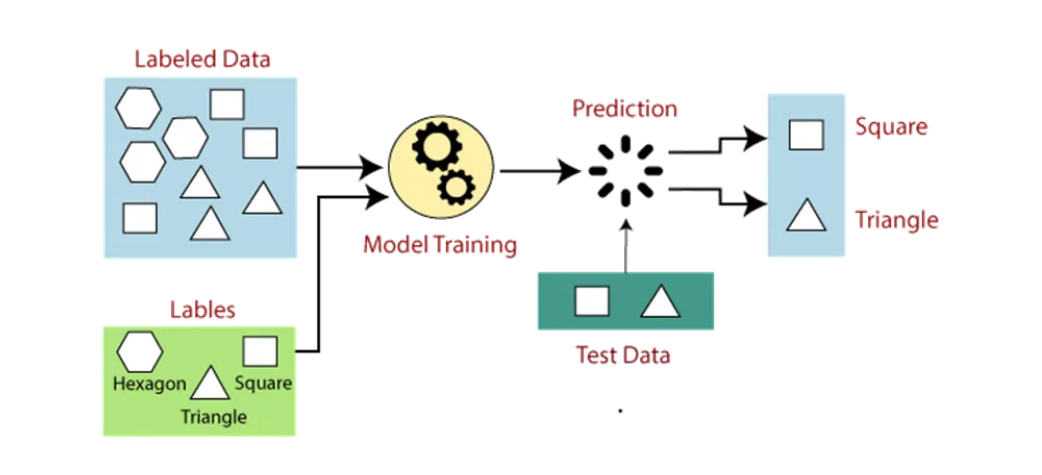
\includegraphics[angle=0, width=\textwidth]{resim1.png}
	
\end{figure} 

\textbf{Denetimsiz Öğrenme Algoritması:} Denetimsiz Öğrenmede ise etiketsiz veriler vardır. Bu etiketsiz veriler arasındaki gizli kalmış yapıyı/örüntüyü bulmaya çalışarak kendi kendine öğrenme biçimi sergilenir.\newline

Denetimli öğrenme genellikle Regresyon ve Sınıflandırma problemlerine uygulanırken, denetimsiz öğrenme Kümeleme (Clustering) ve İlişkilendirme (Association) problemlerine uygulanır.
\begin{figure}[!htbp] 
	\caption{ Denetimsiz Öğrenme  }
	\centering
	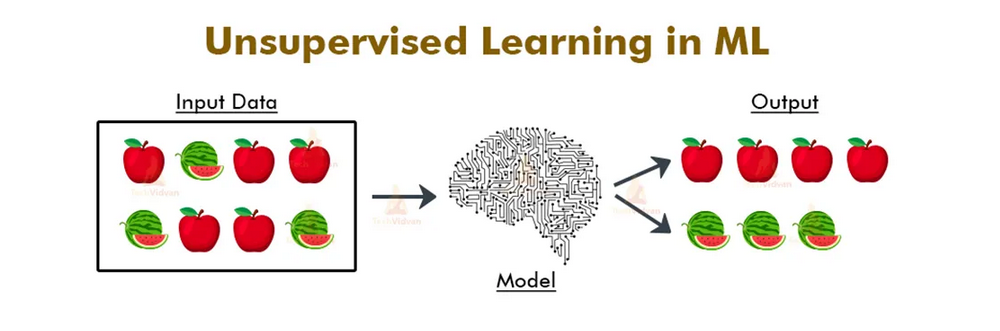
\includegraphics[angle=0, width=\textwidth]{resim2.png}
	
\end{figure} 
\newline
Yukarı da da söylediğimiz gibi Random Fores algoritması araştırıldığında Random Forest regresyon ve Random Forest Sınıflandırma algoritmaları ile karşılaşılacak.Regresyon ve Sınıflandırma algoritmalarına biraz daha açıklık getirmemiz gereklidir.\newline
\textbf{Regresyon(Regression) Nedir ?}


Regresyon bağımlı bir değişken ile bağımsız bir değişken arasındaki ilişkinin, ortadan kaldırılması için kullanılan istatistiksel bir yöntemdir. Evet, regresyonun bu teorik açıklaması size karmaşık gelmiş olabilir. Gelin biz bunu daha basit haliyle açıklayalım. Buradaki değişkenler(x ve y arasında, x → deneyim yılı, y → maaş olarak düşünebilirsiniz) arasında sebep-sonuç ilişkisi bulmaya çalışırız ve bulduğumuz bu ilişkiye göre tahminler yaparız.

En basit haliyle regresyonu açıklayacak olursak, bir veri setinde sayısal tahmin yapıyorsak “regression” algoritmalarını kullanırız.

Örnek → Maaş tahmini, yaşa göre boy tahmini, çalışma süresine göre alınan not tahmini gibi örnekler verebiliriz. \newline

\textbf{Sınıflandırma(Classification) Nedir ?}


Regression problemlerinde tahmin edeceğimiz y kolonunda sayısal değerler vardı. Biz x değerlerini yani giriş değerini kullanarak sayısal tahminler yapmaya çalışıyorduk. Sınıflandırma problemlerinde ise x(giriş değerleri) değerlerini kullanarak kategorik olarak y sınıfını tahmin etmeye çalışırız.\cite{site3}



\begin{figure}[!htbp] 
	\caption{ Regresyon ve Sınıflandırma  }
	\centering
	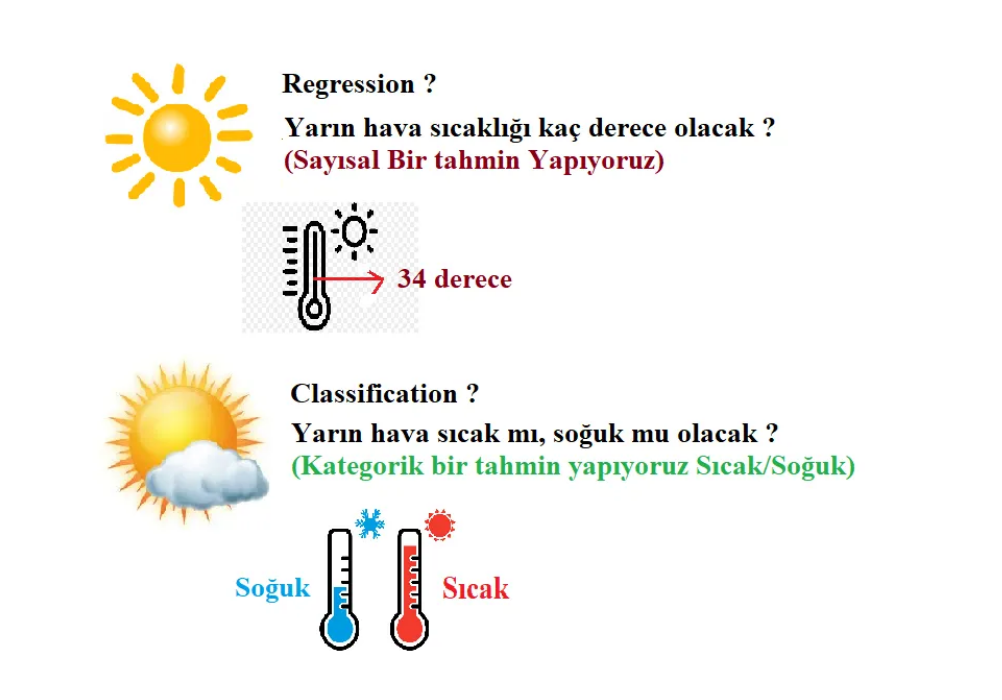
\includegraphics[angle=0, width=\textwidth]{resim4.png}
	\label{dogruluk}
\end{figure} 


\newpage \textbf{Random Forest (Rassal Orman) Algoritması:} 
Sınıflandırma işlemi esnasında birden fazla karar ağacı üreterek sınıflandırma değerini yükseltmeyi hedefleyen bir algoritmadır. Bireysel olarak oluşturulan karar ağaçları bir araya gelerek karar ormanı oluşturur. Buradaki karar ağaçları bağlı olduğu veri setinden rastgele seçilmiş birer alt kümedir.
\begin{figure}[!htbp] 
	\caption{ Single Decision tree and Random Forest }
	\centering
	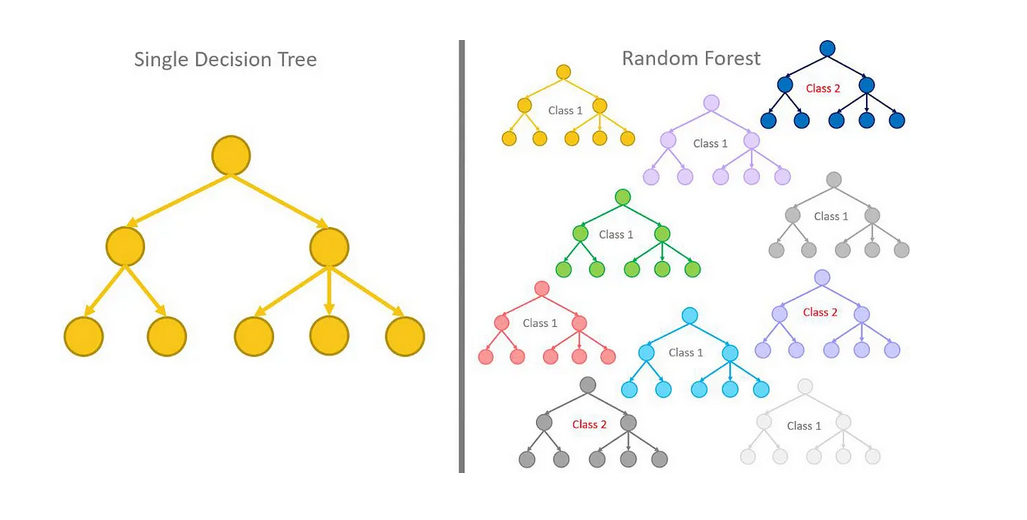
\includegraphics[angle=0, width=\textwidth]{resim5.png}
	
\end{figure} \newline
Fark ettiyseniz Random Forest karar ağaçlarının bir nevi birleşiminden oluşan bir algoritma.\cite{site4}
\newpage


\begin{figure}[!htbp] 
	\caption{ Random Forest }
	\centering
	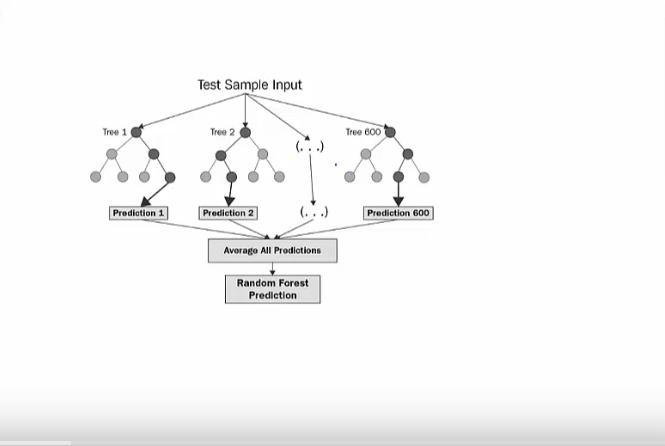
\includegraphics[angle=0, width=\textwidth]{resim6.png}
	
\end{figure} 




\maketitle

Random Forest algoritmamı uygulayacağım veriler aşağıda gösterilmiştir.
\begin{figure}[!htbp] 
	\caption{Covit Verileri}
	\centering
	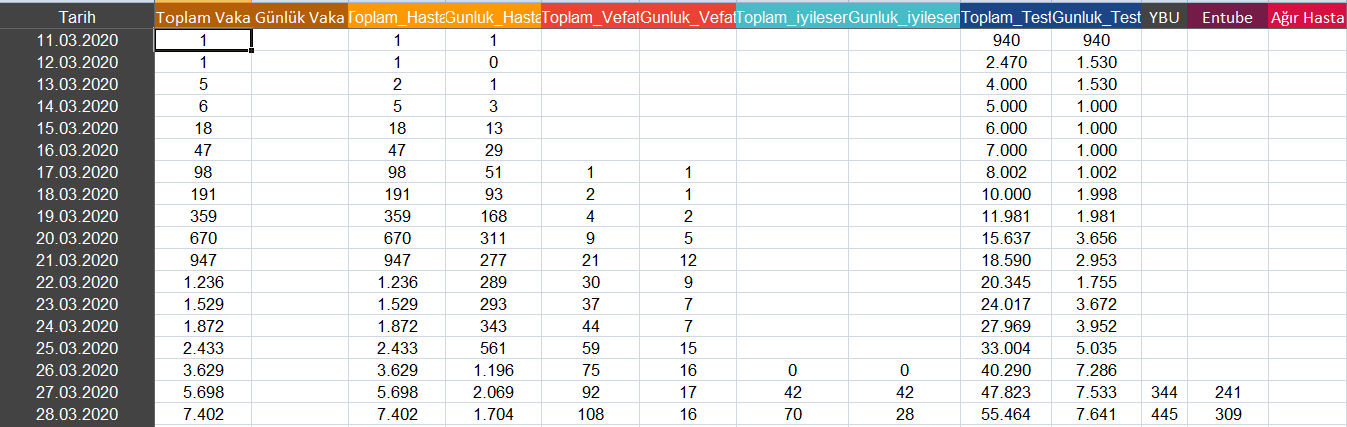
\includegraphics[angle=0, width=\textwidth]{4.0.png}
	
\end{figure} 
\newline
Verilerim gün bazında Türkiye için Toplam Vaka, Günlük Vaka, Toplam Hasta, Günlük Hasta, Toplam Vefat, Günlük Vefat, Toplam İyileşen, Günlük İyileşen, Toplam Test, Günlük Test, Yoğun Bakım Ünitesi ve Ağır Hasta parametrelerinden 812 kayıt içermektedir.

\begin{figure}[!htbp] 
	\caption{Kodlar}
	\centering
	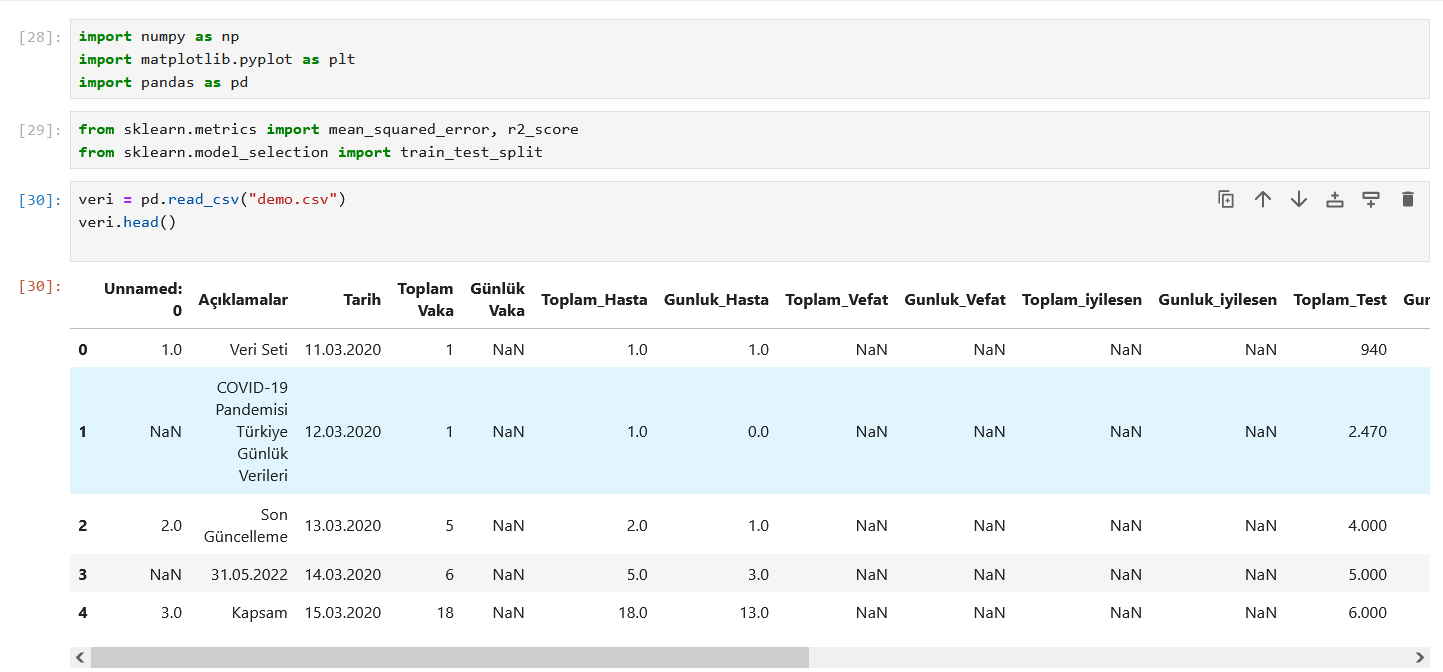
\includegraphics[angle=0, width=\textwidth]{5.0.png}
	
\end{figure} 

Öncelikler kullacağımız kütüpheneleri çalışmamıza ekliyoruz ve pandas kütüphanesinin read.csv fonksiyonuyla verilerimizi içeri alıyoruz.\newline
Daha sonra verilerimizi incelemek ilk 5 veriyi getiriyoruz.

\begin{figure}[!htbp] 
	\caption{Kodlar2}
	\centering
	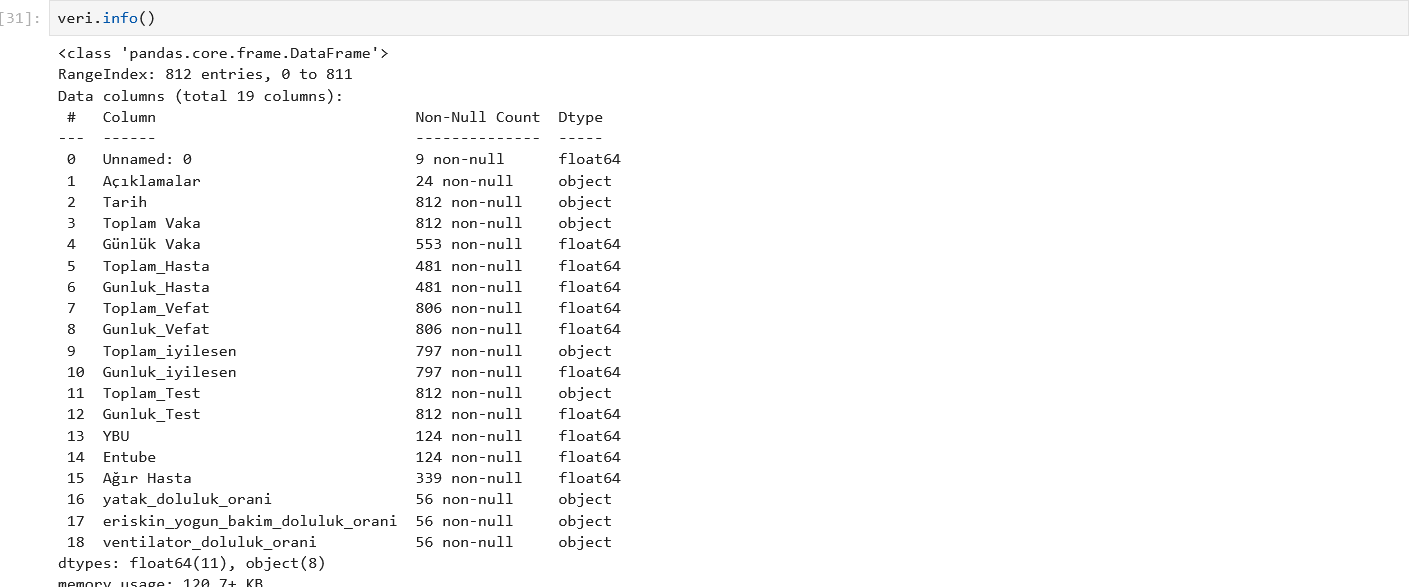
\includegraphics[angle=0, width=\textwidth]{6.0.png} 
	
\end{figure} 
\newpage
Verilerimizi detaylı incelemek için veri.info() metotunu kullanıyoruz.

\begin{figure}[!htbp] 
	\caption{Kodlar3}
	\centering
	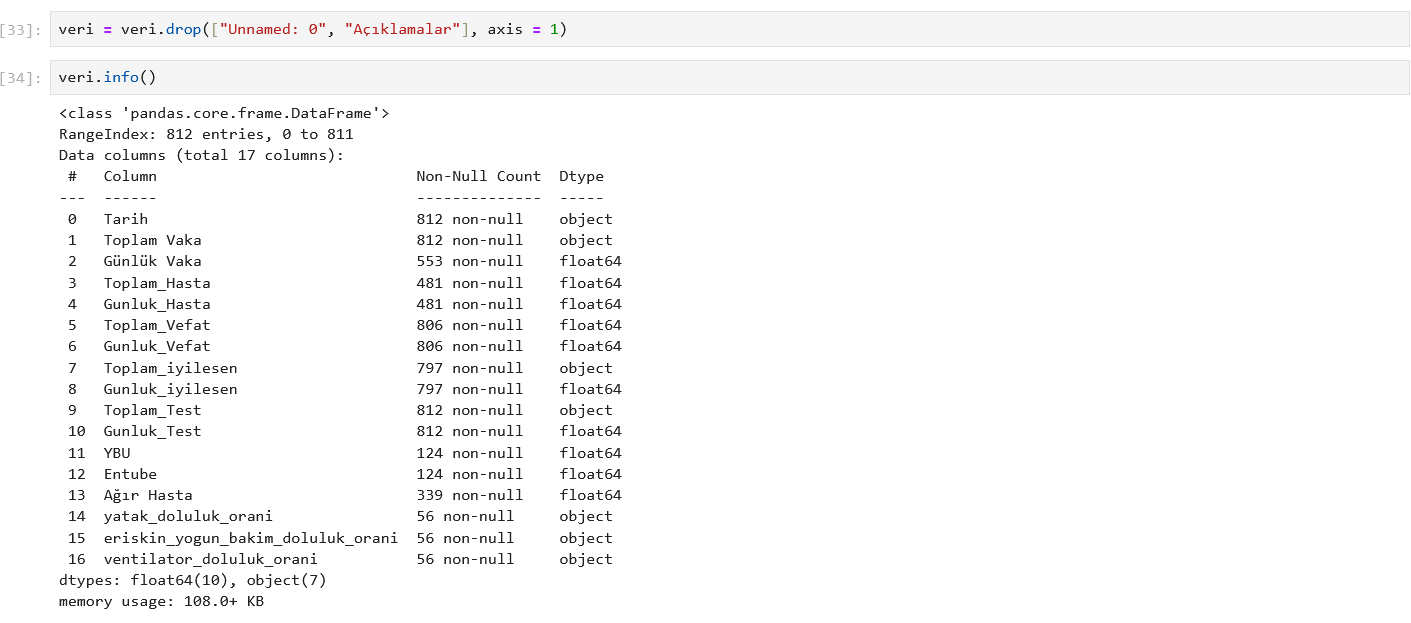
\includegraphics[angle=0, width=\textwidth]{7.0.png} 
	
\end{figure}
Daha sonra kullanılmayacak olan Unnamed : 0 ve Açıklamalar sütununu sililyoruz ve tekrar kontrol ediyoruz.

\begin{figure}[!htbp] 
	\caption{Kodlar4}
	\centering
	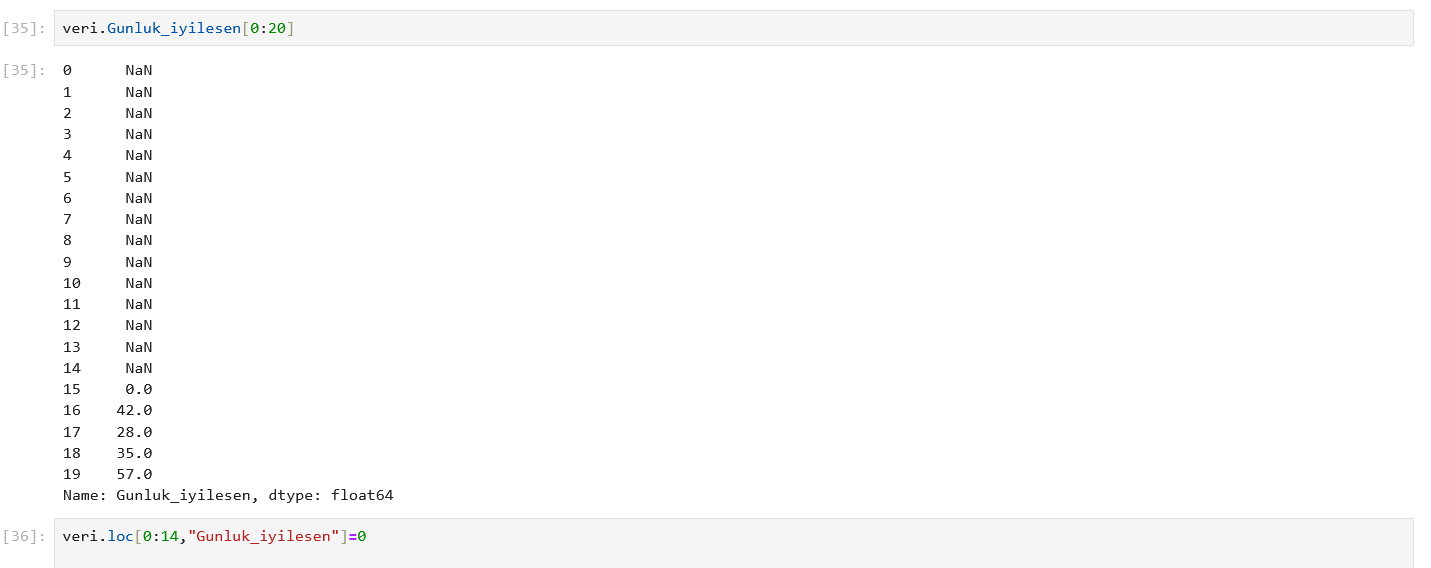
\includegraphics[angle=0, width=\textwidth]{8.0.png} 
	
\end{figure}

\newpage
Günlük iyileşen sütununa baktığımızda ilk 15 verimizin NaN değere sahip olduğunu görüyoruz.Algoritmamızda kullanacağımız için 2 değerini atıyoruz.
\begin{figure}[!htbp] 
	\caption{Kodlar5}
	\centering
	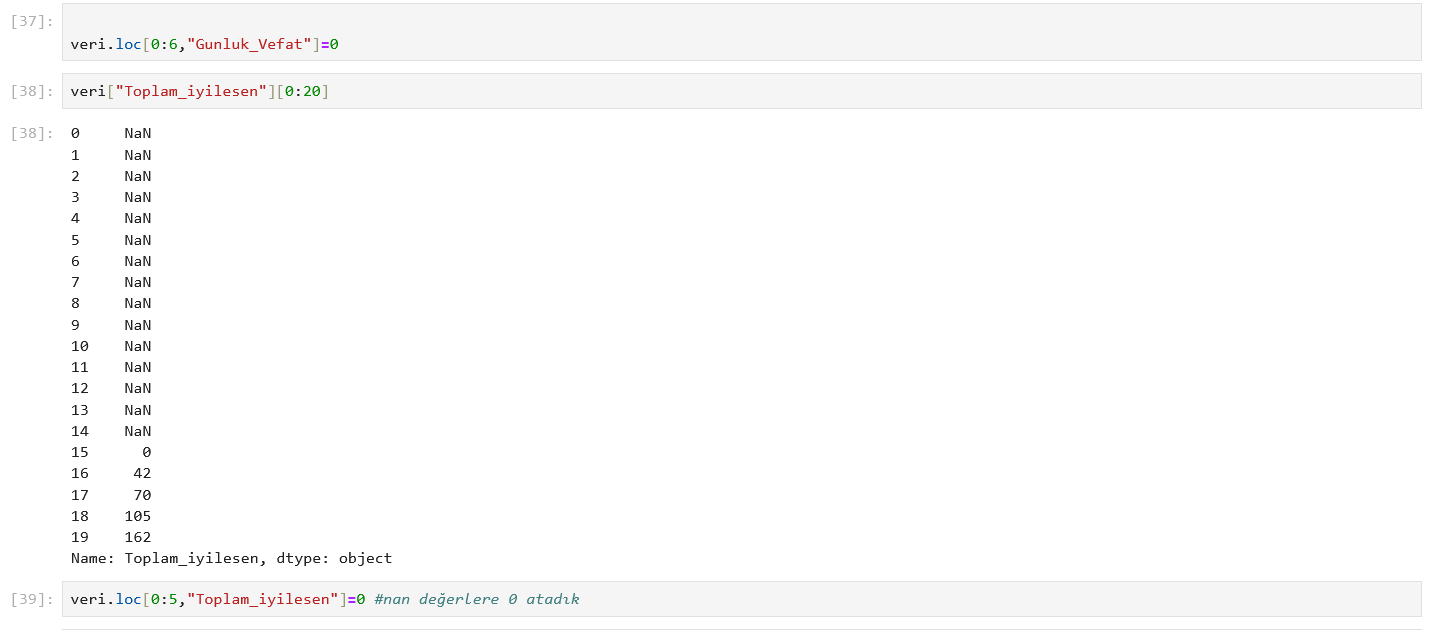
\includegraphics[angle=0, width=\textwidth]{9.0.png} 
	
\end{figure}
Daha sonra aynı işlemi Günlük vefat ve Toplam iyileşen sütunlarımıza da yapıyoruz.

\begin{figure}[!htbp] 
	\caption{Kodlar6}
	\centering
	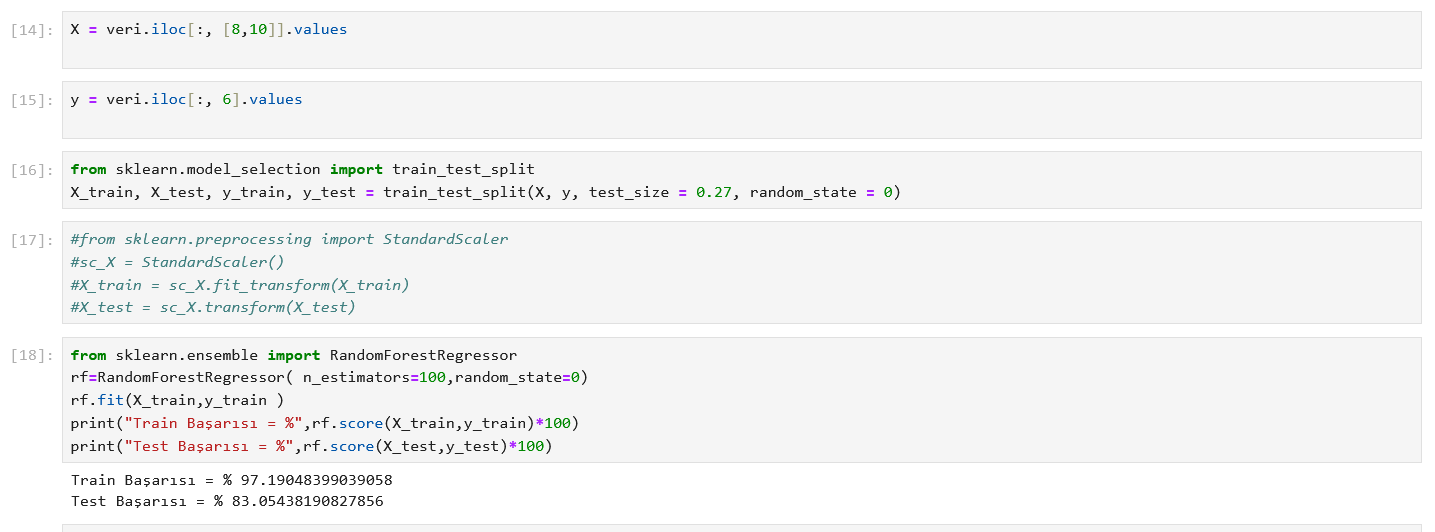
\includegraphics[angle=0, width=\textwidth]{10.0.png} 
	
\end{figure}
\newpage
Daha sonra eğitimde ve testte kullanılacak verilerimizi ayırıyoruz. Verilerimizin \%27 sini test için ayırıyoruz.100 adet karar ağacı kullanıyoruz.Eğitim başarımını \%97 test başarımını \%83 olarak buluyoruz.

\begin{figure}[!htbp] 
	\caption{Kodlar7}
	\centering
	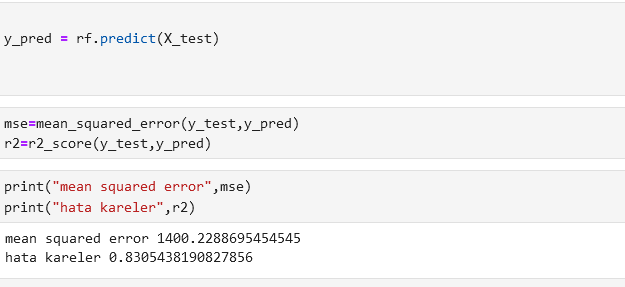
\includegraphics[angle=0, width=\textwidth]{11.0.png} 
	
\end{figure}
\textbf{R Kare:} R kare, modeldeki bağımsız değişkenlere göre bağımlı değişkenin varyasyon oranını yani bağımlı değişkendeki değişkenliğin ne kadarının model tarafından açıklanabileceğini ölçer. Korelasyon katsayısının karesidir. R Kare aşırı uyum (overfitting) sorununu dikkate almaz. Regresyon modelinin çok fazla bağımsız değişkeni varsa model eğitim verilerine çok iyi uyabilir ama testte istenen başarıyı gösteremeyebilir. Bu nedenle Düzeltilmiş R Kare kullanılır. Düzeltilmiş R Kare modele eklenen ek bağımsız değişkenleri cezalandırır ve aşırı uyum sorununu çözer.\newline
\begin{math} 
	\centering	\newline 1-\frac{Ssres}{SStot} 
\end{math}\newline
SSres: hata kareler toplamı\newline
SStot: toplam kareler toplamı\newline
\textbf{Ortalama Kare Hatası (Mean Squared Error (MSE)):} Ortalama Kare Hatası tahmin edilen sonuçlarınızın gerçek sayıdan ne kadar farklı olduğuna dair size mutlak bir sayı verir. Tek bir sonuçtan çok fazla içgörü yorumlayamazsınız, ancak size diğer model sonuçlarıyla karşılaştırmak için gerçek bir sayı verir ve en iyi regresyon modelini seçmenize yardımcı olur. \cite{site11}
\begin{math} 
	\centering	\newline \frac{1}{n} * \sum_{}^{}(y-ypred)^2
\end{math}	
\newline n:Veri noktalarının sayısı.
\newline y:Gerçek değerler.
\newline ypred: Tahmin edilen değerler.
\newline Daha Sonraki projemizi diğer veri setinden çektiğimiz veriler ile yapacağız.\cite{owidcoronavirus}
\begin{figure}[!htbp] 
	
	\centering
	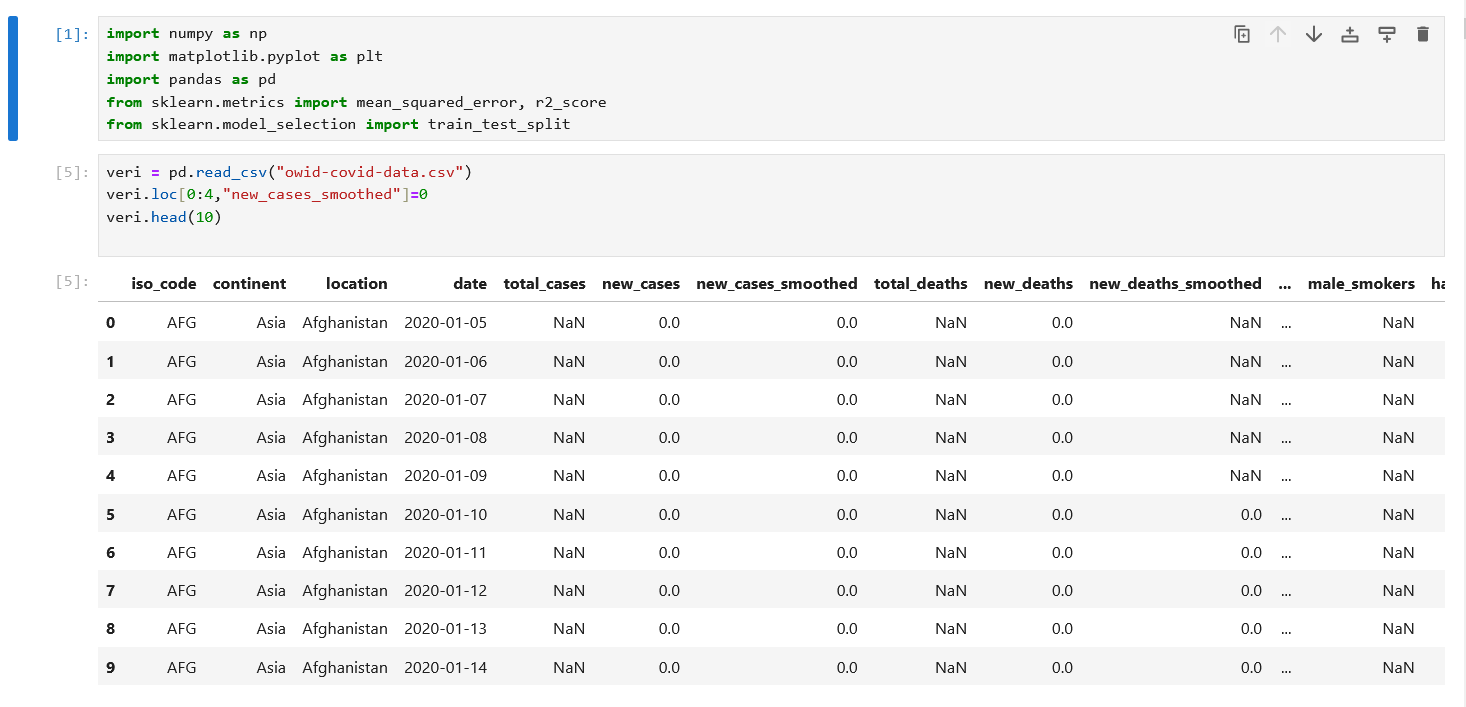
\includegraphics[angle=0, width=\textwidth]{1.png}
	\caption{Verilemizin Genel İncelenmesi}
	
	
\end{figure} 
\newline   Yukarıda gördüğünüz kodlarda kullanıcağımız kütüphaneleri projemize ekledik ve kullanacağımız verilerden new cases smoothed sütunundaki ilk 4 veri NaN değere sahip olduğu için 0 atadık ve daha sonra ilk 10 verimizi kontrol ettik.
\begin{figure}[!htbp] 
	
	\centering
	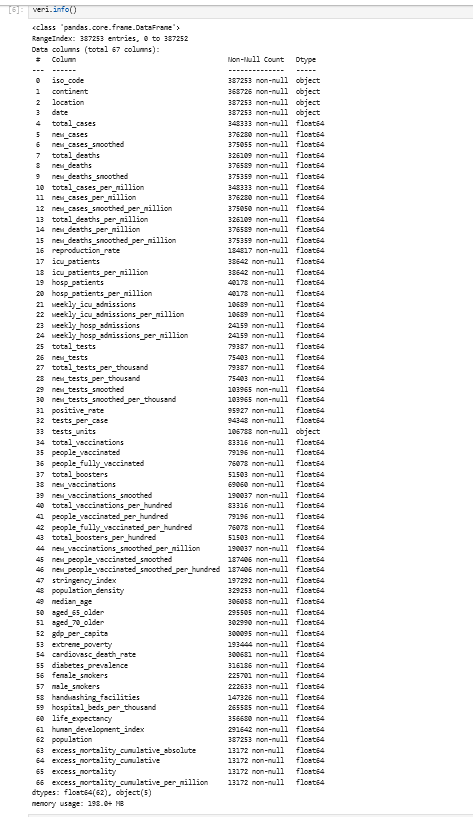
\includegraphics[angle=0, width=\textwidth]{2.png}
	\caption{Verilerimize Detaylı İncelenmesi}
\end{figure}
\newpage Hangi türden ne kadar veri olduğunu ve hangi sütun adı altında olduklarını inceledik. 
\begin{figure}[!htbp] 
	
	\centering
	
\includegraphics[angle=0, width=\textwidth]{3.png}
	\caption{Afganistan için new cases sütununun seçilmesi}
\end{figure}
\newline İlk verilerimiz Afganistan'a ait verilerdir.Verilerimizi bir dataframe a atıp location kolonunda Afghanistan olan verilerimizi alıyoruz(Birden fazla ülkenin verileri aynı veri tabanında olduğu için).Daha sonra bağımlı değişkenlerimizde kullanmak  üzere new cases verilemizi ayıklayıp indeks numarası 7 nin katları olacak şekilde tekrar alıyoruz.Bunun sebebi ise verilerimizin her 7 günde güncellenmesi aradaki günlerde veri girilmemesi.
\begin{figure}[!htbp] 
	
	\centering
	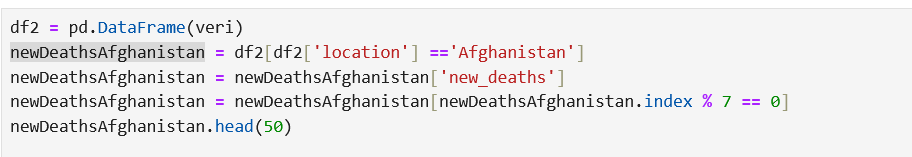
\includegraphics[angle=0, width=\textwidth]{4.png}
	\caption{Afganistan için new deaths sütununun seçilmesi}
\end{figure}
\newline Aynı işlemleri new deaths, new cases smoothed, diabetes prevalence, cardiovasc death rate ve population sütunlarımız içinde yapıyoruz.
\begin{figure}[!htbp] 
	
	\centering
	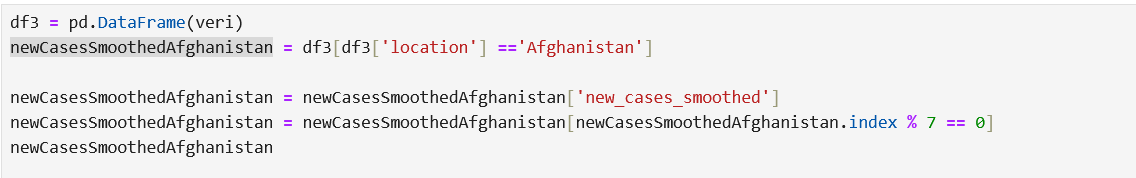
\includegraphics[angle=0, width=\textwidth]{5.png}
	\caption{Afganistan için new cases smoothes sütununun seçilmesi}
\end{figure}
\begin{figure}[!htbp] 
	
	\centering
	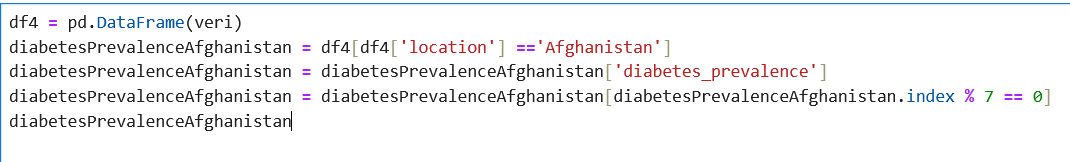
\includegraphics[angle=0, width=\textwidth]{6.png}
	\caption{Afganistan için diabetes prevalance sütununun seçilmesi}
\end{figure}
\begin{figure}[!htbp] 
	
	\centering
	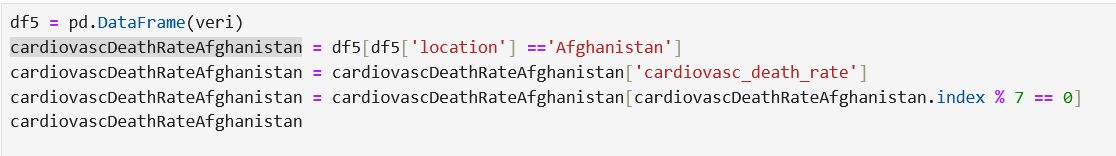
\includegraphics[angle=0, width=\textwidth]{7.png}
	\caption{Afganistan için cardiovasc death rate sütununun seçilmesi}
\end{figure}
\begin{figure}[!htbp] 
	
	\centering
	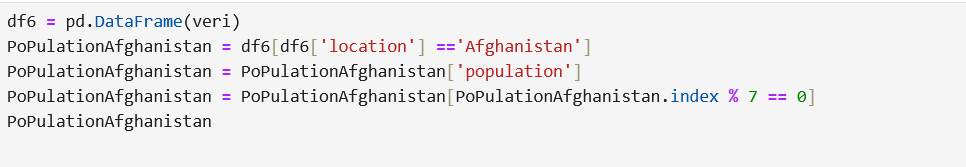
\includegraphics[angle=0, width=\textwidth]{8.png}
	\caption{Afganistan için population sütununun seçilmesi}
\end{figure}
\begin{figure}[!htbp] 
	
	\centering
	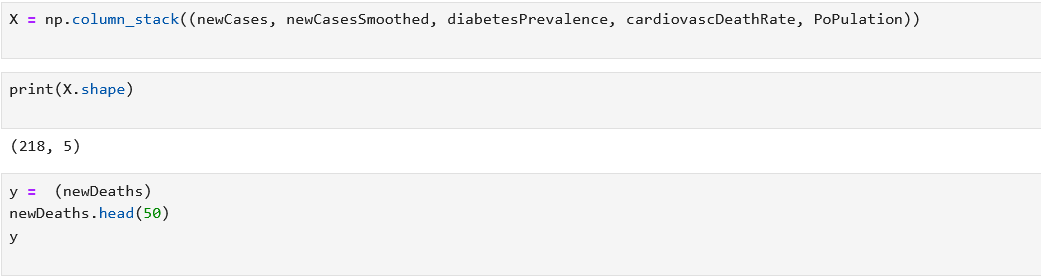
\includegraphics[angle=0, width=\textwidth]{9.png}
	\caption{Bağımlı ve bağımsız değişkenlerin oluşturulması}
\end{figure}
\newline
\newpage
Daha sonra projemizde kullanmak üzere bağımlı X ve bağımsız y değikenlerini oluşturuyoruz.Kodda da görüldüğü gibi bağımlı değişkenimiz new cases, new cases smoothed, diabetes prevalence, cardiovasc death rate ve population verilerimiz içerirken tahim edeceğimiz yani bağımsız değişkeinimiz new deaths verilerini içeriyor.En son olarak bağımlı ve bağımsız değişkenlerin boyutlarını kontrol etmemin sebebi satır sayılarının aynı olması gerektiğindendir.
\newline
\begin{figure}[!htbp] 
	
	\centering
	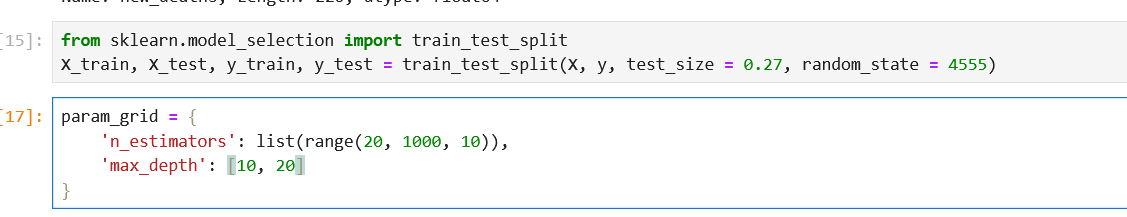
\includegraphics[angle=0, width=\textwidth]{10.png}
	\label{fig:yenietiket}
	\caption{Test, eğitim verilerinin ayrılması ve parametre ayarı.}
\end{figure}
\newline Yukarıdaki kodda test ve eğitim verilerimizi \%27 test verisi olacak şekilde ayırdık.Daha sonra en başarılı parametre ayarını bulmak için değişkenlerimizi tanımladık.

\begin{figure}[!htbp] 
	
	\centering
	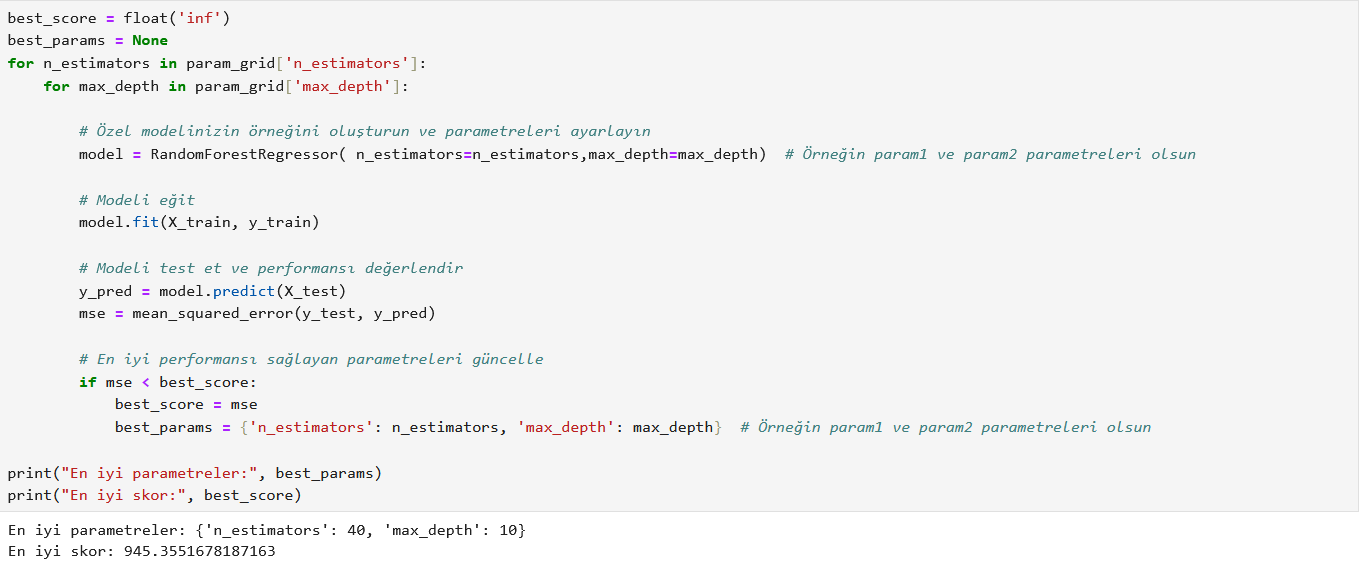
\includegraphics[angle=0, width=\textwidth]{11.png}
	\label{fig:yenietiket2}
	\caption{Test, eğitim verilerinin ayrılması ve parametre ayarı.}
\end{figure}
Yukarıdaki kodda Resim \ref{fig:yenietiket} da tanımladığımız değişkenleri kullanarak her değişkenin tüm kombinasyonlarını deneyerek mse sini hesaplıyoruz ve en skoru veren parametre değerlerini buluyoruz.


\begin{figure}[!htbp] 
	
	\centering
	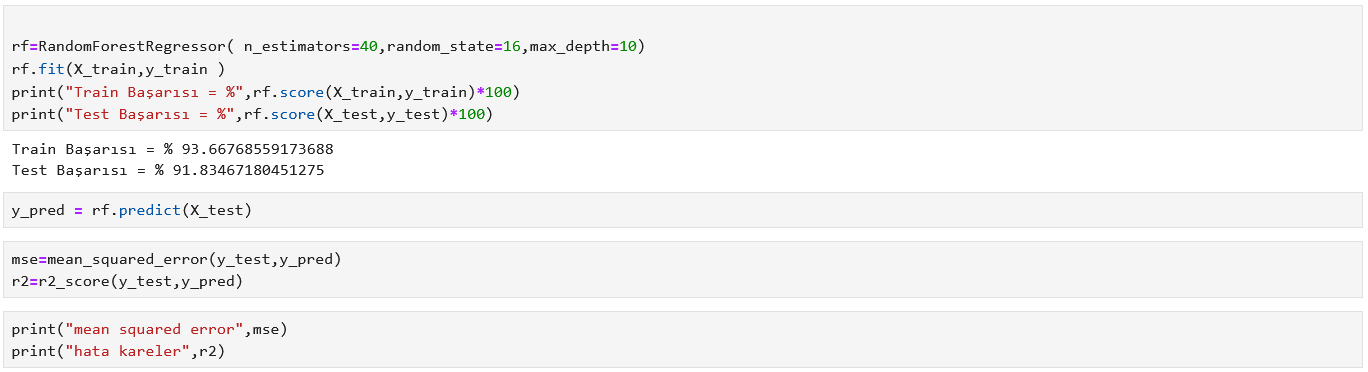
\includegraphics[angle=0, width=\textwidth]{13.png}
	\caption{Modelin eğitilmesi.}
\end{figure}
\newpage
En son olarak Resim \ref{fig:yenietiket2} de elde ettiğimiz verilere göre modelimizi eğitiyoruz, mse ve r2 değerlerini hesaplıyoruz.
\newline
\newline
Aynı işlemi veri tabanımızdaki Avustralya, Brezilya, ve Çin içinde yaptık.Lakin eğitim başarımları ve test başarımları tatmin edici seviyede değildi.

\begin{figure}[!htbp] 
	
	\centering
	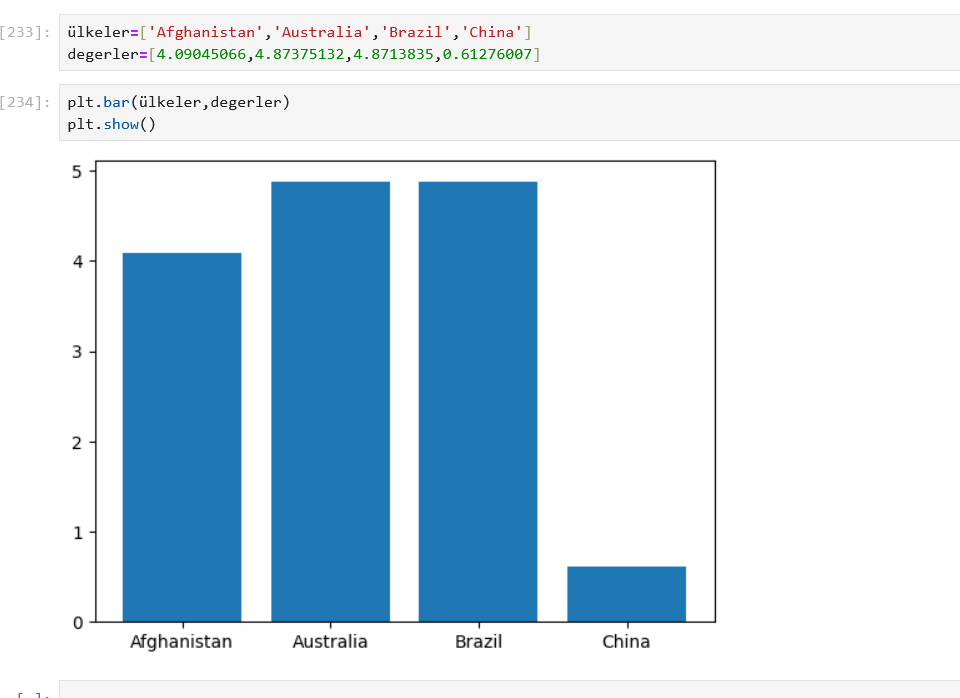
\includegraphics[angle=0, width=\textwidth]{14.png}
	\caption{4 Ülkenin Karşılaştırılması.}
\end{figure}
Yukarıdaki kodlarda 4 ülke için eğitilmiş modele beslediğimiz değerlerden (new cases = 100 ,new cases smoothed = 20, diabetes prevalence = 5, cardiovasc death rate=150, population = 1000000) elde ettiğimiz çıktılar karşılaştırılmıştır.
\newline
\begin{centering}
	
\begin{tabular}{lll}
	\hline
	Ülkeler  & Eğitim başarımı & Test başarımı \\ \hline
	Afghanistan & \% 93.66 & \% 91.83 \\
	Australya1 & \% 87.35 & \% 35.51 \\
	Brezil & \% 93.18 & \% 54.74 \\
	China & \% 78.92 & \% 57.72 \\
	\hline
\end{tabular}
\end{centering}
\newline Yukarıdaki tabloda projemde kullandığım ülke verilerin eğitim ve test başarımları verilmiştir.

\bibliographystyle{ieeetr}
\bibliography{document_vize.bib}





\end{document}
